%!TEX root = ../thesis.tex

\chapter{Methodology}
\label{ch:met}

This study employs the COMER methodology for the generation of test cases.
In order to assess the efficacy of the framework and conduct comparative analyses with other existing frameworks, I undertook the task of implementing it from scratch using the Python programming language.
The initial implementation by Niu \textit{et al.} \cite{comer} was coded in Java.
However, this implementation presented certain limitations; the code was compiled into a jar file, making it challenging to extend or modify functionalities.
Consequently, I opted to develop my own implementation in Python, making necessary modifications to facilitate experimentation with different datasets and enhancing the usability of the framework.
Python was chosen due to its user-friendly syntax and the availability of extensive libraries for data manipulation and visualization.


\section{COMER Framework}\label{sec:comer-framework}

The COMER framework serves the purpose of generating test cases, leveraging both traditional Combinatorial Testing (CT) methods and incorporating metamorphic relations during the generation process.
Upon receiving inputs including a set of metamorphic relations, a set of constraints, and abstract input parameters, COMER generates test cases that adhere to the specified constraints while satisfying certain metamorphic relations.

The framework operates in two primary stages:

\subsection{Abstract Test Case Generation}\label{subsec:abstract-test-case-generation}

The algorithm for abstract test case generation encompasses two main pathways.
At each step, there exists a probability distribution determining the choice between two flows.
In the first flow, the algorithm functions akin to a conventional CT generation algorithm, employing a greedy approach to generate test cases until achieving the desired t-way coverage.
Conversely, the second flow involves the selection of a previously generated test case, followed by the generation of subsequent test cases utilizing metamorphic relations. The second flow works by running Constrain Satisfaction Solver to produce follow up test cases giver previous test case, constraints, parameters and metamorphic relations.

\subsection{Concrete Test Case Generation}\label{subsec:concrete-test-case-generation}

Subsequently, the generated abstract test cases are mapped to concrete ones.
For test cases generated via CT methods, the concrete test case is produced by randomly selecting a value from the domain corresponding to the abstract value.
Conversely, for test cases generated through metamorphic relations, the framework utilizes the specified MRs to generate subsequent test cases. Full example of generating test cases from inputs is shown at Fig.~\ref{fig:comer_example}

\begin{figure}[hbt]
    \centering
    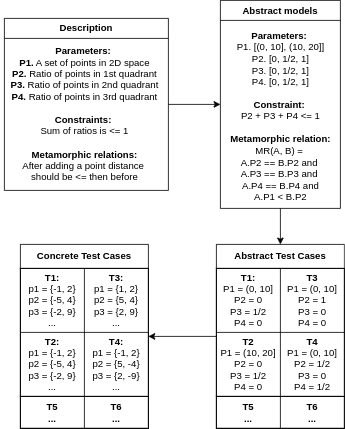
\includegraphics[]{figs/test_cases.png}
    \caption{Example of generating test cases for \textit{FindClosest} function. Note that $T1$ and $T2$ are parameters generated by utilizing MR.}
    \label{fig:comer_example}
\end{figure}


\section{Limitations}\label{sec:limitations}

Despite the advancements made in the original COMER implementation, certain limitations were identified.
Firstly, the reliance on a greedy approach for generating Combinatorial Testing (CT) test cases posed a notable drawback.
While this method can increase the speed of generation process, it may result in an excessive number of test cases, potentially compromising efficiency and resource utilization.
Secondly, the focus of the implementation solely on metamorphic relations with a single input and a single follow-up test case restricted its applicability to scenarios involving more complex MRs. Thirdly, the lack of provision for generating test cases for functions beyond those already supported in the implementation posed a significant constraint.

In my implementation, efforts were made to mitigate some of these limitations.
To overcome the limitation of supporting only a limited range of functions, I worked to improve the framework by allowing the generation of test cases for any function.
Additionally, in response to concerns regarding the effectiveness of the greedy approach, provisions were made to incorporate alternative algorithms for CT test case generation, thereby offering users flexibility in selecting the most suitable approach.
However, it is important to note that the limitation pertaining to MRs with multiple inputs and follow-up test cases remains unaddressed in my implementation, representing an area for potential future research and improvement.

\section{Vulnerability Selection}\label{sec:vulnerability-selection}

This study utilizes the OWASP Top 10 vulnerabilities to assess the effectiveness of COMER framework in identifying and testing for common web application vulnerabilities. The OWASP Top 10 is a widely recognized list of the most critical security risks facing web applications \cite{OWASP}. 

Among the OWASP Top 10 vulnerabilities, I selected Injection as the primary testing scenario. Injection attacks involve injecting malicious code or data into an application's inputs in order to extract sensitive information, manipulate database queries, or execute arbitrary commands.

Injection is a particularly critical vulnerability due to its high potential impact and widespread prevalence in web applications. The OWASP Top 10 highlights injection attacks as one of the top 10 most critical security risks facing web applications. The goal of this paper is to test specifically SQL injections and general injection attacks, such as buffer overflow and input sanitization. 

\subsection{Test Case Generation}\label{sec:test-case-generation}

To test for SQL Injection vulnerabilities, I employed the COMER framework to generate test cases using existing combinatorial input space \cite{SQLInjection}. This approach involved generating a comprehensive set of input values that satisfied various metamorphic relations.

The generated test cases were designed to mimic real-world user inputs and simulate malicious injection attacks. The framework's ability to incorporate metamorphic relations enabled the generation of test cases that effectively targeted SQL Injection vulnerabilities.

\subsection{Metamorphic Relations}\label{sec:metamorphic-relations}

The metamorphic relations employed in this study were designed to simulate various injection attack scenarios. They enabled the generation of different SQL statements by manipulating the input data, while the combinatorial part was used mostly to escape and bypass sanitization mechanisms.

These relations allowed me to manipulate the input data in such a way that different SQL statements could be generated, while still maintaining a realistic and comprehensive set of test cases.

\section{App selection}\label{sec:app-selection}

For this study, I selected two web-based applications that are widely used in the field of penetration testing and vulnerability assessment. The chosen applications are:

\begin{itemize}
	\item \textbf{WebGoat}: A web-based application security testing platform that allows users to simulate various types of attacks. \cite{Webgoat}

	\item \textbf{DVWA (Damn Vulnerable Web Application)}: A deliberately vulnerable web application designed for testing and training purposes. \cite{DVWA}
\end{itemize}

These two applications were selected because they provide a comprehensive set of vulnerabilities and functionalities, making them suitable for testing the COMER framework. The use of these applications will allow me to demonstrate the effectiveness of the COMER framework in generating test cases that can identify and exploit various types of security vulnerabilities.

\section{Metrics}

In order to measure the effectiveness of proposed approach different metrics were chosen:

\begin{itemize}
	\item \textbf{Detection rate}: Measures the ability of the COMER framework to accurately identify and flag vulnerabilities within the selected web applications. This metric is fundamental in determining the effectiveness of the framework in identifying security threats.
	\item \textbf{Generation Time Efficiency}: Quantifies the speed and computational resources required by the COMER framework to generate test cases and identify vulnerabilities. This metric is essential for evaluating the practicality and scalability of the approach in real-world scenarios.
	\item \textbf{Number of test cases}: Similar to \textbf{Generation Time Efficiency}, but quantifies speed of test execution instead of generation. An excessively large number of test cases may also lead to increased testing overhead and resource consumption. 
\end{itemize}

Several widely used metrics, like test coverage, were omitted due to the specifics of web security testing. In many instances, accessing the web application's code is not feasible. As a result, metrics suitable for a black box approach were utilized instead.